% ME4370 - Mechatronics - Tristan Hill
% Guest Lecture - March 2, 0216

% Timing - MCUs and PCs - Deterministic vs. Non Deterministic 

% Document settings
\documentclass[11pt]{article}
\usepackage[margin=1in]{geometry}
\usepackage[pdftex]{graphicx}
\usepackage{multirow}
\usepackage{setspace}
\usepackage{hyperref}
\usepackage{color,soul}
\usepackage{fancyvrb}
\usepackage{amsmath}
\usepackage{amssymb}
\usepackage{multicol}

\pagestyle{plain}
\setlength\parindent{0pt}
\hypersetup{
bookmarks=true,         % show bookmarks bar?
unicode=false,          % non-Latin characters in Acrobat’s bookmarks
pdftoolbar=true,        % show Acrobat’s toolbar?
pdfmenubar=true,        % show Acrobat’s menu?
pdffitwindow=false,     % window fit to page when opened
pdfstartview={FitH},    % fits the width of the page to the window
pdftitle={My title},    % title
pdfauthor={Author},     % author
pdfsubject={Subject},   % subject of the document
pdfcreator={Creator},   % creator of the document
pdfproducer={Producer}, % producer of the document
pdfkeywords={keyword1} {key2} {key3}, % list of keywords
pdfnewwindow=true,      % links in new window
colorlinks=true,       % false: boxed links; true: colored links
linkcolor=red,          % color of internal links (change box color with linkbordercolor)
citecolor=green,        % color of links to bibliography
filecolor=magenta,      % color of file links
urlcolor=blue           % color of external links
}


\newcommand{\HSIZ}{3mm}
\newcommand{\VSIZ}{3mm}

\begin{document}
    
	\textbf{\LARGE ME 4370 - Mechatronics - Spring 2016}\\\\
	\textbf{\LARGE {\it It is all about it Timing - PCs vs. MCUs}}\\
	    \begin{description}
        \item[\textbf{Overview}]\textbf{:}\\\\
        
            A microcontroller, or MCU is fundamentally different from a personal computer. MCUs are capable of operating on {\it precise} timing rountines while personal computers run on a {\it non-deterministic} timing. Therefore, one specialized capability of an MCU is precise timing of input and output as well as internal events. Personal computers cannot do this. 
        
        \item[\textbf{Measure Time}]\textbf{:}\\    
            
            How could we make a timer? Lets talk about some ideas. 
                \begin{enumerate}
                    \item moon and stars (sun)
                    \item seasons
                    \item sand, hourglass
                    \item pendulum, time based on $\omega_n$ powered by weight or springs
					\item quartz or other crystall based timing
					\item whats another oscillator you can think of?
                \end{enumerate}
            
		\item[\textbf{The System Clock}]\textbf{:}\\ 
			
			Most MCUs contain an internal oscillator based on a quartz crystal (\href{https://en.wikipedia.org/wiki/Crystal_oscillator}{wikipedia}). This oscillator is used as the {\it system clock} which schedules program execution and allows for advanced timing capabilties. The speed of this system is often measured in MIPS (Million Instructions Per Second) not to be confused with (Microprocessor without Interlocked Pipeline Stages).\\
			
			We generally do not interface the system clock directly, however there is a specialized register that we can access called the timer counter TCNT. Our MCU (ATMEGA2560) has several of these available. If the timer counter is enabled it acts as a {\it free running timer}. It is really just a register that increments itself in time with the system clock.\\
			
			Consider the 8bit timer counter TCNT0 on your 16MHz ATMEGA2560. What does this mean? This means that on every cycle of the clock TCNT0 = TCNT0 + 1. However we do not see this in code. This happens very quickly! So to use it to measure events that that more than a very short time we have to manage the {\it timer overflow}. It turns out there is a register for that.
			
			
            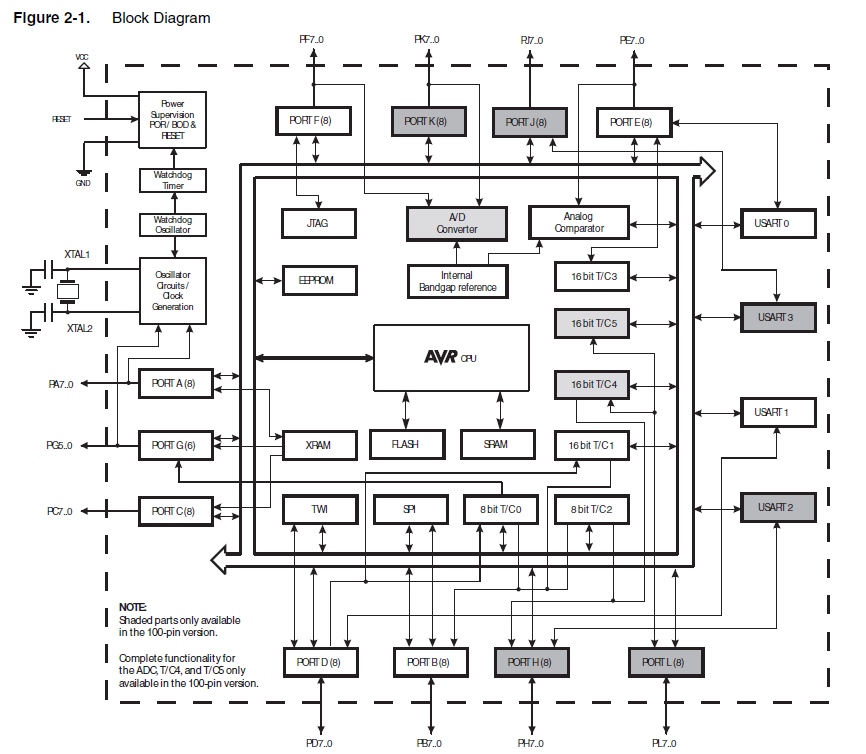
\includegraphics[scale=.75]{timer_fig1.png}
			
			
        \item[\textbf{Timing on a PC}]\textbf{:}\\  
		
		Why does it take so long for a to PC application to load? PCs also operate on a very similar system clock. The main difference is the fact an OS level computer is doing many things at once and the multiple routines and programs must share the system resources. So scheduling these events in true real time is a very difficult task but it can be done (RTOS). Alternatively, most OS have {\it non-deterministic} timing routines. 

\newpage
        
		\item[\textbf{Precise Timing Capabilities}]\textbf{:}\\  
			
			\begin{enumerate}
				\item Scheduling Internal Events
				\item Timing Internal Events
				\item Scheduling External Events - Outputs
				\item Timing External Events - Inputs 	\\
			\end{enumerate}
		
		\item[\textbf{Scheduling Internal Events}]\textbf{:}\\ 
			
		Scheduling internal events using the TCNT register is generally done through {\it polling} or through the use of {\it interrupt routines}. 
		
		Polling is act of accessing the TCNT register, and this is generally in the main code, {\it loop}. The example shows a while loop used to wait until the TCNT register reaches a certain value. This may be the easiest way the do internal timing but it is not the best.\\ 
		
			\textbf{Polling example 2 }
		\begin{verbatim}
			
			void loop() {
  
  c_time=TCNT1L;
  
  while (!(TCNT0<200);
  c_cnt++;

  Serial.println(c_cnt);
  
  
}
		\end{verbatim}
			
		\textbf{Polling example 2 }
		\begin{verbatim}
			
			void loop() {

  c_time=TCNT1L;
  
  while (!(TIFR1&B00000001));
  c_cnt++;

  Serial.println(c_cnt);
  
  
}
		
			
		\end{verbatim}
		
		\newpage
		Interrupt Service Routines encompass are a very important capability of the MCU. An ISR or referred to as an {\it Interrupt} is a special block of code, i.e. a function, that executes exactly when we need it to. This can be based on different things, but in this example the function {\it fires} whe TCNT reaches a certain value. This is commonly referred to as a {\it Real Time Interrupt}.
		\textbf{ISR example}
		\begin{verbatim}
		void setup()
{     
pinMode(13,OUTPUT);
/* or use:
DDRB = DDRB | B00100000;  // this sets pin 5  as output
                       // without changing the value of the other pins 
*/
// Disable interrupts while loading registers
cli();
// Set the registers
TCCR1A = 0; //Timer Counter Control register
// Set mode
TCCR1B = (1 << WGM12); // turn on CTC mode
// Set prescale values (1024). (Could be done in same statement
// as setting the WGM12 bit.)
TCCR1B |= (1 << CS12) | (1 << CS10);
//Enable timer compare interrupt===> TIMSK1 for ATmega328, 
//TIMSK for ATmega8
TIMSK |= (1 << OCIE1A);
// Set OCR1A
OCR1A = 15624;
// Enable global interrupts
sei();
}
void loop(){}

ISR (TIMER1_COMPA_vect) {
   digitalWrite(13, !digitalRead(13));
   //PORTB ^= _BV(PB5); // as digitalWrite(13,x) is an Arduino 
   //function, direct writing to the port may be preferable
}
		\end{verbatim}
		
		
    \end{description}
\end{document}



